\documentclass[10pt]{beamer}
\usepackage{lmodern}
\usepackage{amsmath}
\usefonttheme{structurebold}
\usetheme{Rochester}

\usepackage[backend=biber]{biblatex}

\addbibresource{presentation.bib}

\setbeamertemplate{navigation symbols}{\insertlogo}

\begin{document}
\author{Thu-Ngan Doan, Hoang-Quan Tran, Tan-Tho Huynh, Nhat-Dang Su, Diem-Uyen Phan-Dang}
\title{Efficiency of the Simplex Method}
\subtitle{Investigating on how fast Simplex Method will solve a problem in a given size.}
\logo{
\includegraphics[scale=.2]{img/fithcmuslogo.png}}
\institute{VNUHCM - University of Science}
\date{Spring 2022}
\subject{CSC10104 - Linear Programming}

\setbeamercovered{transparent}
\setbeamertemplate{navigation symbols}{}

\begin{frame}[plain]
\maketitle
\end{frame}

\begin{frame}
\frametitle{Table of Contents}
\tableofcontents
\end{frame}

\section{Introduction}
\begin{frame}{Introduction}

\end{frame}

\section{Performance Measures}
\begin{frame}{Performance Measures}
Can be divied into two types:
\begin{itemize}
\item Worst case: asking how much efforts is needed to solve all problems of a given \textit{size}
\item Average case: looking at the average amount of effort, averaging over all problems of a giving \textit{size}. 
\end{itemize}
Worst-case analyses are generally easier than Average-case.
\end{frame}

\section{Measuring the Size of a Problem}
\begin{frame}{Measuring the Size of a Problem}

\end{frame}

\section{Measuring the Effort to Solve a Problem}
\begin{frame}{Measuring the Effort to Solve a Problem}

\end{frame}

\section{Worst-case Analysis of the Simplex Method}
\begin{frame}{Worst-case Analysis of the Simplex Method}
\begin{itemize}
\item The upper bound of basic feasible solutions is $\displaystyle {n + m \choose n}$.
\item For a fixed value of the sum $n + m$, this expression is maximized when $m = n$.
\item Hence, we can easily estimate an upper and lower bound of $\displaystyle {2n \choose n}$\cite{Vanderbei2020}:
$$
\frac{2^{2n}}{2n} \leq {2n \choose n} \leq 2^{2n} \ (n \in \mathbb{N^+})
$$
\end{itemize}
\end{frame}
\begin{frame}{Worst-case Analysis of the Simplex Method (cont.) - Proof}
\begin{theorem}[Stirling's approximation\cite{weisstein}]
$$
\displaystyle
n! \operatorname*{\sim}_{n\to\infty} \sqrt{2\pi n}\left(\frac{n}{e}\right)^n
$$
\end{theorem}
Given that $\displaystyle {2n \choose n} = \frac{(2n)!}{(n!)^2}$\footnote{${n \choose k} = \frac{n!}{(n - k)!k!}$} and following expressions:
\begin{itemize}
\item $\displaystyle (2n)! \operatorname*{\sim}_{n\to\infty} 2\sqrt{\pi n} \left(\frac{2n}{e}\right)^{2n}$ 
\item $\displaystyle (n!)^2 \operatorname*{\sim}_{n\to\infty} 2\pi n \left(\frac{n}{e}\right)^{2n}$ 
\end{itemize}
Hence, $\displaystyle {2n \choose n} \operatorname*{\sim}_{n\to\infty} \frac{2\sqrt{\pi n} \left(\frac{2n}{e}\right)^{2n}}{2\pi n \left(\frac{n}{e}\right)^{2n}} =  \frac{2^{2n}}{\sqrt{\pi n}}$
\end{frame}

\begin{frame}{Worst-case Analysis of the Simplex Method (cont.) - Proof}
\begin{proof}
Let
$$
\displaystyle
L = \frac{\frac{2^{2n}}{2n}}{\frac{2^{2n}}{\sqrt{\pi n}}} = \frac{2^{2n}\sqrt{\pi n}}{2^{2n} 2n} = \frac{\sqrt{\pi}}{2} \frac{1}{\sqrt{n}} < 1,\ \forall n \in \mathbb{N^+}
$$
Since $L < 1$, we can state that $\frac{2^{2n}}{2n} \leq \frac{2^{2n}}{\sqrt{\pi n}},\ \forall n \in \mathbb{N^+}
$
. Hence,
$$
\displaystyle
\frac{2^{2n}}{2n} \leq \frac{2^{2n}}{\sqrt{\pi n}} \leq 2^{2n} \iff \frac{2^{2n}}{2n} \leq {2n \choose n} \leq 2^{2n}
$$
\end{proof}
This states that in the worst case, the algorithm has the complexity of $\Theta(2^{2n})$. $2^{2n}$ is huge even though $n$ is \textit{not} very big. (e.g with $n = 25$, $2^{50} = 1.1259\times 10^{15}$)
\end{frame}

\begin{frame}{Worst-case Analysis of the Simplex Method (cont.) - Example}
In 1972, V. Klee and G.J. Minty\cite{klee1970good} were the first to discover an example in which the
simplex method using the largest coefficient rule requires $2^n - 1$ iterations to solve:
\begin{equation*}
\sum_{j = 1}^{n} 2^{n - j} x_j \rightarrow \max
\end{equation*}
subjects to
\begin{equation*}
\begin{aligned}
2\sum_{j = 1}^{i - 1} 2^{i - j}x_j + x_i &\leq 100^{i - 1} & (i = 1, 2, .., n)\\
x_j &\geq 0 & (j = 1, 2, .., n)
\end{aligned}
\end{equation*}
\end{frame}

\begin{frame}{Worst-case Analysis of the Simplex Method (cont.) - Example}
If we look closely, the first 3 constraints are:
\begin{equation*}
\begin{aligned}
x_1 &\leq 1\\
4x_1 + x_2 &\leq 10^2\\
8x_1 + 4x_2 + x_3 &\leq 10^4
\end{aligned}
\end{equation*}
These constraints are just simply a set of upper bounds. The feasible region is now a stretched $n$-dimensional hypercube:
\begin{equation*}
\begin{aligned}
0 \leq x_1 &\leq 1\\
0 \leq x_2 &\leq 100\\
&\vdots\\
0 \leq x_n &\leq 100^{n - 1}
\end{aligned}
\end{equation*}
\end{frame}

\begin{frame}{Worst-case Analysis of the Simplex Method (cont.) - Example}
This feasible region for the Klee-Minty problem is often referred as the Klee-Minty cube\footnote{more percisely, a hyperrectangle}.
\begin{figure}
	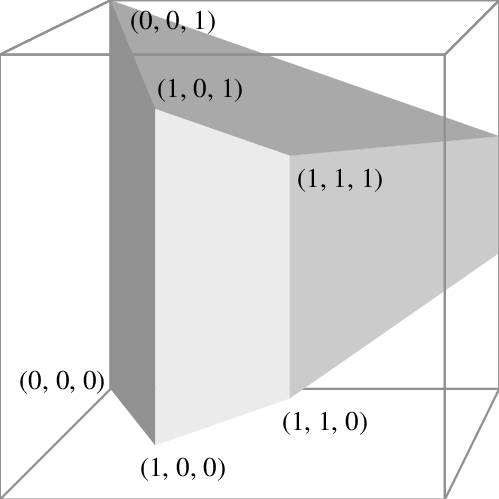
\includegraphics[scale=.2]{img/klee-minty-cube.png}
	\caption{Klee-Minty cube with $n = 3$ and $\epsilon = \frac{1}{3}$}
\end{figure}
An $n$-dimension hypercube has $2^n$ vertices.
\end{frame}


\section{Empirical Average Performance of the Simplex Method}
\begin{frame}{Empirical Average Performance of the Simplex Method}

\end{frame}

\section{References}
\begin{frame}[allowframebreaks]{References}
\printbibliography
\end{frame}
\end{document}
